The {\em echoc} module provides echo cancellation. As a non-adaptive method, it operates in two phases: In the measurement phase, a test signal is played back through the speaker outputs \attr{loudspeakerports} and the response is recorded through the microphone inputs \attr{micports}. In the filter phase, the output signals are filtered with the phase-inverted corresponding responses, and the signal is added to the microphone signal. An overview of the signal flow is given in the figure \ref{fig:modechoc}.

Please note that no feedback jack connections are possible for the echo cancellation to work, because feedback connections cause an additional delay which results in a mismatch of the cancellation signal. This also means that a graph from the microphone to the loudspeaker (e.g., self monitoring) is not possible for the echo cancellation to work. Future versions may compensate for this extra delay.

The filter is implemented in frequency domain as overlap-save algorithm.

\begin{figure}[htb]
    \centering
    \fbox{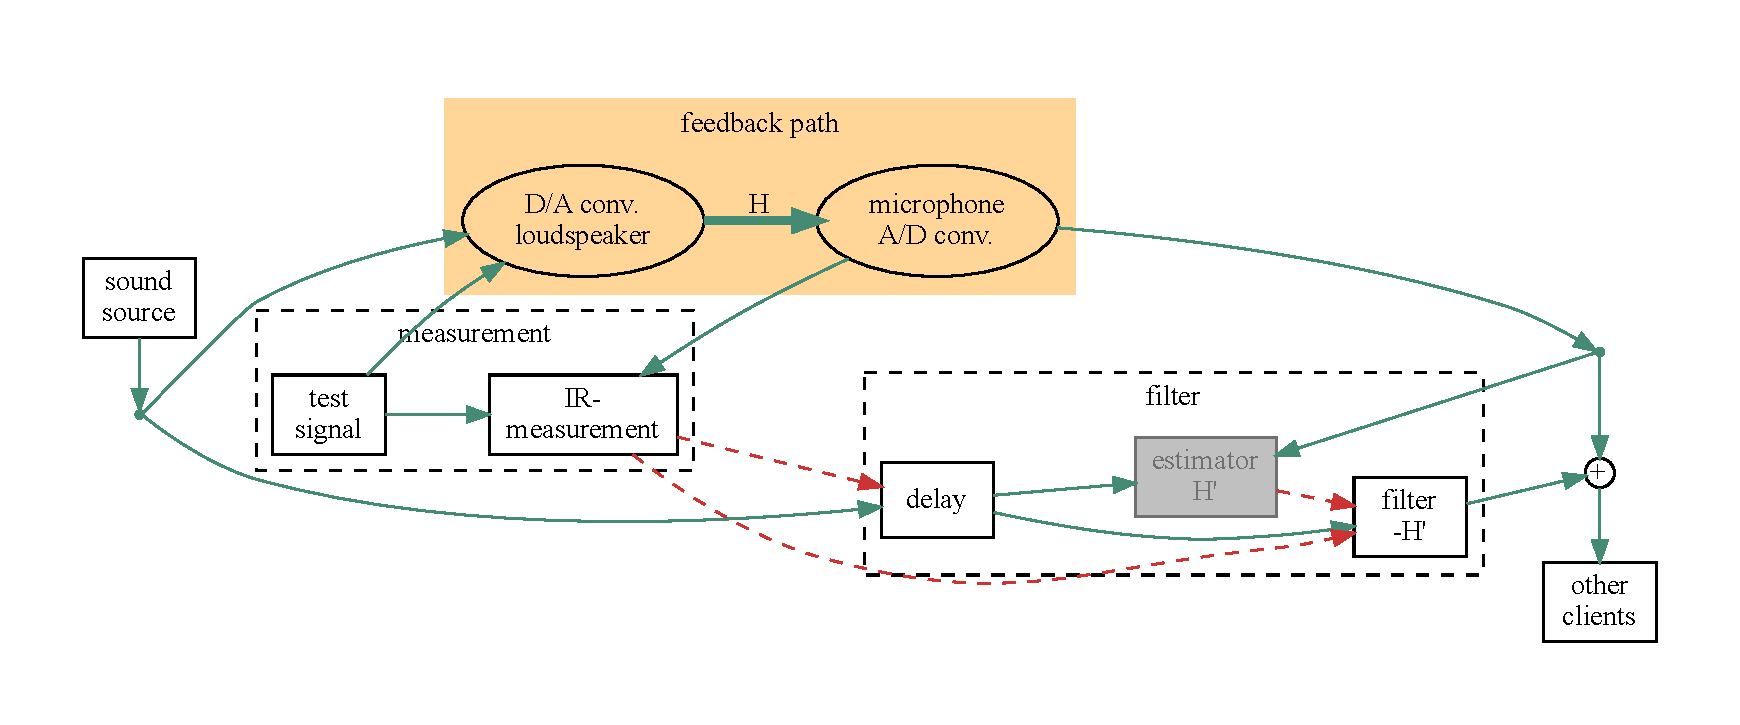
\includegraphics[width=\textwidth]{echoc.pdf}}
    \caption{Signal flow of the echoc plugin. The sound source (left side) is played back through the loudspeakers. In the signal sent to the other clients (on the right side), the sound source is cancelled. The adaptive filter estimator (gray box) is not yet implemented.}
    \label{fig:modechoc}
\end{figure}



\begin{snugshade}
{\footnotesize
\label{attrtab:echoc}
Attributes of element {\bf echoc}\nopagebreak

\begin{tabularx}{\textwidth}{lXl}
\hline
name & description (type, unit) & def.\\
\hline
\hline
\indattr{autoreconnect} & Automatically re-connect ports after jack port change (bool) & false\\
\hline
\indattr{bypass} & Bypass filter stage (bool) & false\\
\hline
\indattr{filterlen} & Minimal length of filters (uint32, samples) & 65\\
\hline
\indattr{level} & Playback level (float, dB SPL) & 70\\
\hline
\indattr{loudspeakerports} & Loudspeaker ports (string array) & {\tiny system:playback\_1 system:playback\_2}\\
\hline
\indattr{maxdist} & Maximum distance between microphone and loudspeaker (float, m) & 2\\
\hline
\indattr{measureatstart} & Perform a measurement when the plugin is loaded (bool) & false\\
\hline
\indattr{micports} & Microphone ports (string array) & system:capture\_1\\
\hline
\indattr{name} & Client name, used for jack and IR file name (string) & echoc\\
\hline
\indattr{nrep} & Number of measurement repetitions (uint32) & 16\\
\hline
\indattr{premax} & Time before to maximum to add to filter (uint32, samples) & 8\\
\hline
\end{tabularx}
}
\end{snugshade}
